\section{Teoremi della divergenza e del rotore}
\subsection{Lemma di Green}
In questa sezione vengono richiamati i teoremi della divergenza e del rotore, già incontrati nei corsi di Analisi. Viene introdotto il teorema del gradiente. Questi teoremi vengono dimostrati a partire da due lemmi, che risultano utili nella scrittura delle equazioni di bilancio di un continuo (solido o fluido che sia). Il punto di partenza è il lemma di Green, necessario per la dimostrazione dei due lemmi. La sua dimostrazione viene riportata per motivi di completezza e per richiamare alcuni concetti già incontrati nei corsi di Analisi e per ricominciare ad utilizzarli.

\begin{theorem}[Lemma di Green]\label{thm:green}\index{Lemma di Green}
Sia $\gamma_R$ una curva chiusa semplice nel piano positivamente orientata regolare a tratti, e sia $R$ la superficie di cui è frontiera. Se $P$ e $Q$ sono due funzioni reali di due variabili reali che hanno le derivate parziali continue su una regione aperta che contiene $R$.
%\centering
\begin{equation}\label{eqn:green_thm} 
\begin{aligned}
 \iint_R \frac{\partial P}{\partial y} dx dy  = 
   - \oint_{\gamma_R} P dx,  \quad
  \iint_R \frac{\partial Q}{\partial x} dx dy = 
    \oint_{\gamma_R} Q dy
\end{aligned}
\end{equation}
\end{theorem}
%
La dimostrazione viene svolta prima per domini semplici, come il dominio $R$ in figura \ref{fig:green}, e poi generalizzata per domini non semplici e non semplicemente connessi.
\begin{remark}
 Il verso positivo di percorrenza di una linea chiusa nel piano è quello antiorario, come indicato in figura \ref{fig:green}: seguendo questa convenzione, la regione limitata del piano viene lasciata a sinistra della curva, se percorsa nel verso positivo.
\end{remark}

\begin{proof}
Se $R$ è un dominio semplice, è possible dimostrare la prima delle due equazioni (\ref{eqn:green_thm}) scomponendo il contorno $\gamma_R = \partial R$ nelle due curve $\ell_1: y=Y_1(x)$ e $\ell_2: y=Y_2(x)$, come in figura \ref{fig:green}. \'E possibile scrivere il contorno $\gamma_R = \ell_1 \cup \ell^{-}_2$ come unione delle due curve $\ell_1$ ed $\ell_2$, dove l'apice $^{-}$ su $\ell_2$ indica che deve essere percorsa per $x$ decrescenti affinché il contorno $\gamma_R$ sia percorso in senso positivo.
%
%Andando da $x=a$ a $x=b$ lungo $Y_2(x)$ si percorre il contorno $\gamma_R$ in senso antiorario (positivo), mentre andando da $x=a$ a $x=b$ lungo $Y_1(x)$ si percorre il contorno $\gamma_R$ in senso orario (negativo).
%
\begin{equation}
\begin{aligned}
  \iint _R \frac{\partial P}{\partial y} dx dy = 
  \int_{a}^{b} \displaystyle \left(\int_{Y_1(x)}^{Y_2(x)} \frac{\partial P}{\partial y} dy \right) dx = 
 \int_{a}^{b} \left[ P(x,Y_2(x)) - P(x,Y_1(x)) \right] dx = - \oint_{\gamma_R} P dx
\end{aligned}
\end{equation}
%
In maniera analoga, è possibile dimostrare la seconda delle (\ref{eqn:green_thm}), scomponendo il contorno in due curve $\ell_1: x=X_1(y)$ e $\ell_2: x=X_2(y)$, con $X_2(x) > X_1(x)$.
%
\begin{equation}
\begin{aligned}
  \iint _R \frac{\partial Q}{\partial x} dx dy = 
  \int_{e}^{f} \displaystyle \left(\int_{X_1(y)}^{X_2(y)} \frac{\partial Q}{\partial x} dx \right) dy = 
 \int_{e}^{f} \left[ P(X_2(y),y) - P(X_1(y),y) \right] dy = \oint_{\gamma_R} Q dy
\end{aligned}
\end{equation}
%
\end{proof}
%
%%\begin{wrapfloat}{figure}{r}{0pt}\label{fig:green}
%\begin{figure}\label{fig:green}
%  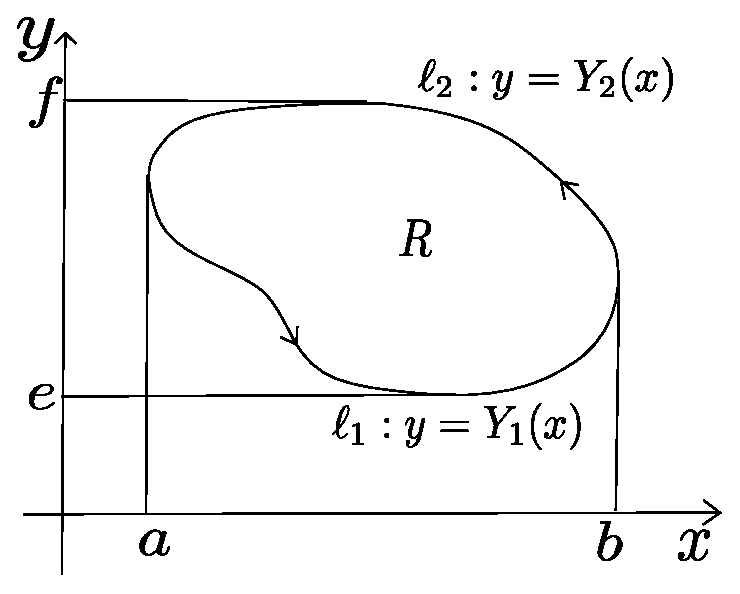
\includegraphics[width=0.40\textwidth]{./fig/green}
% \caption{Dominio semplice $R$}
%\end{figure}
%%\end{wrapfloat}
%
Sottraendo le due equazioni del teorema \ref{thm:green}, si ottiene la forma classica nella quale il teorema di Green viene presentato
\begin{equation}
   \oint_{\gamma_R} [P dx + Q dy] = 
  \iint_R \displaystyle\left( \frac{\partial Q}{\partial x} - \frac{\partial P}{\partial y} \right) dx dy .
\end{equation}
%


\paragraph{Domini non semplici e non semplicemente connessi.}
Il caso di domini non semplici e non semplicemente connessi si riconduce al caso di domini semplici, in seguito all'introduzione
di un 'taglio' $\gamma_c$ nel dominio, sfruttando la regolarità (per ipotesi) della funzione all'interno del dominio.
 Nel caso di dominio non semplice, ci si riconduce a due o più domini semplici a due a due disgiunti, la cui unione è l'insieme 
non semplice di partenza. Nel caso di dominio non semplicemente connesso, ci si riconduce al caso di dominio semplicemente 
connesso.

Nel caso di dominio non semplice, si ha:

\begin{equation}
\begin{aligned}
  \iint_R \frac{\partial P}{\partial y} dx dy & = & \text{($R = R_1 \cup R_2$)} \\
  & = \iint_{R_1} \frac{\partial P}{\partial y} dx dy + \iint_{R_2} \frac{\partial P}{\partial y} dx dy = & \text{($l_1 = \partial R_1$, $l_2 = \partial R_2$)} \\
  & = - \oint_{l_1} P dx - \oint_{l_2} P dx = & \text{($l_1 = \gamma_1 \cup \gamma_c$ , $l_2 = \gamma_2 \cup \gamma_c^{-}$)} \\
  & = - \int_{\gamma_1} P dx - \int_{\gamma_c} P dx - \int_{\gamma_c^{-}} P dx - \int_{\gamma_2} P dx = & 
  \text{$\displaystyle\left(\int_{\gamma_c^{-}} P dx = -\int_{\gamma_c} P dx ,  \right.$} \\
  & & \text{$ \gamma_1 \cup \gamma_2 = \partial R = \gamma \bigg)$}
 \\
  & = -\oint_\gamma P dx
\end{aligned}
\end{equation}

\begin{figure}[h]
\centering
%\captionsetup[subfigure]{labelformat=empty}
\subfloat[][\emph Dominio non semplice $R = R_1 \cup R_2$. Il taglio $\gamma_c$ viene percorso in entrambi i versi e per questo dà contributo nullo: negli integrali viene indicato con $\gamma_c$ quando fa parte del contorno $l_1$ e con $\gamma_c^{-}$ quando fa parte del contorno
$l_2$ e viene percorso nel verso contrario.]
   {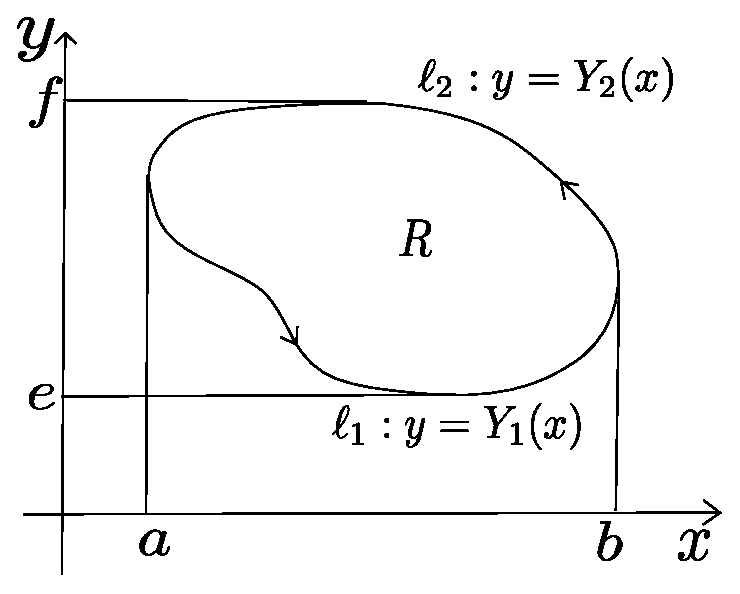
\includegraphics[width=0.30\textwidth]{./fig/green.eps}} \quad
\subfloat[][\emph Dominio non semplice $R = R_1 \cup R_2$. Il taglio $\gamma_c$ viene percorso in entrambi i versi e per questo dà contributo nullo: negli integrali viene indicato con $\gamma_c$ quando fa parte del contorno $l_1$ e con $\gamma_c^{-}$ quando fa parte del contorno
$l_2$ e viene percorso nel verso contrario.]
   {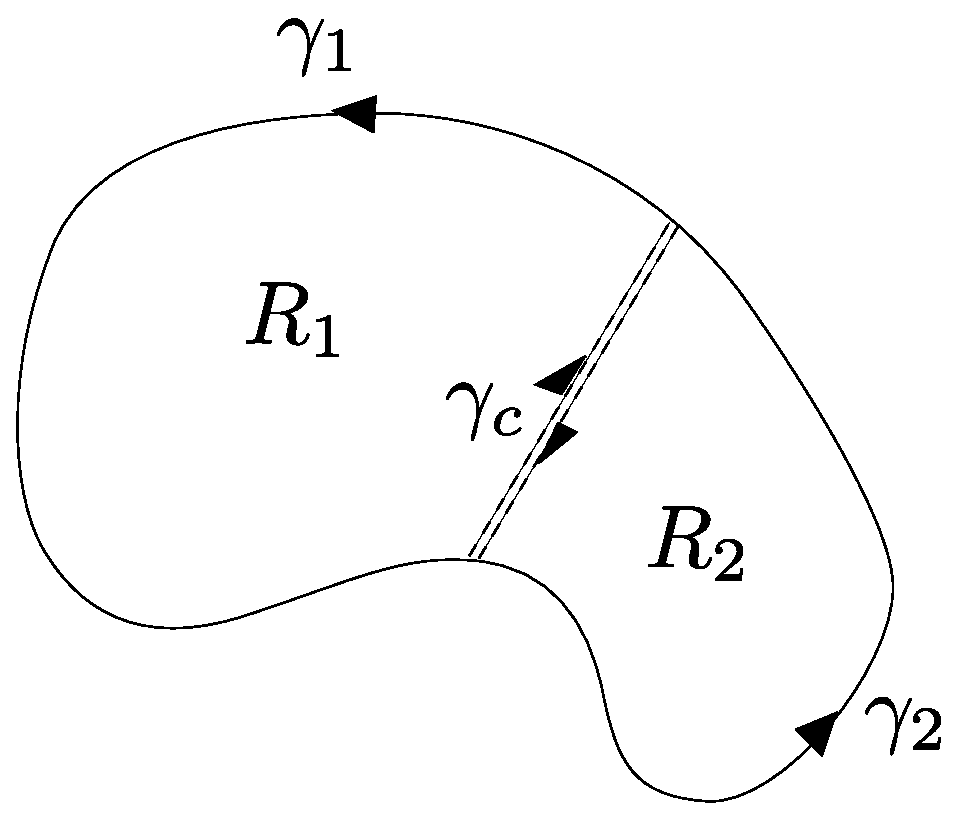
\includegraphics[width=0.30\textwidth]{./fig/nonSempl.eps}} \quad
\subfloat[][\emph Dominio non semplicemente connesso $R$. I contributi calcolati sul 'taglio' sono opposti e quindi si annullano.
   Il contorno del dominio $R$ è costituito da $\gamma_1$ e $\gamma_2$: si osservi che $\gamma_1$ è percorso in senso antiorario, mentre
   $\gamma_2$ in verso orario, concorde con la convenzione che il verso positivo di percorrenza del contorno è quello che lascia sulla
   sua sinistra il dominio. ]
   {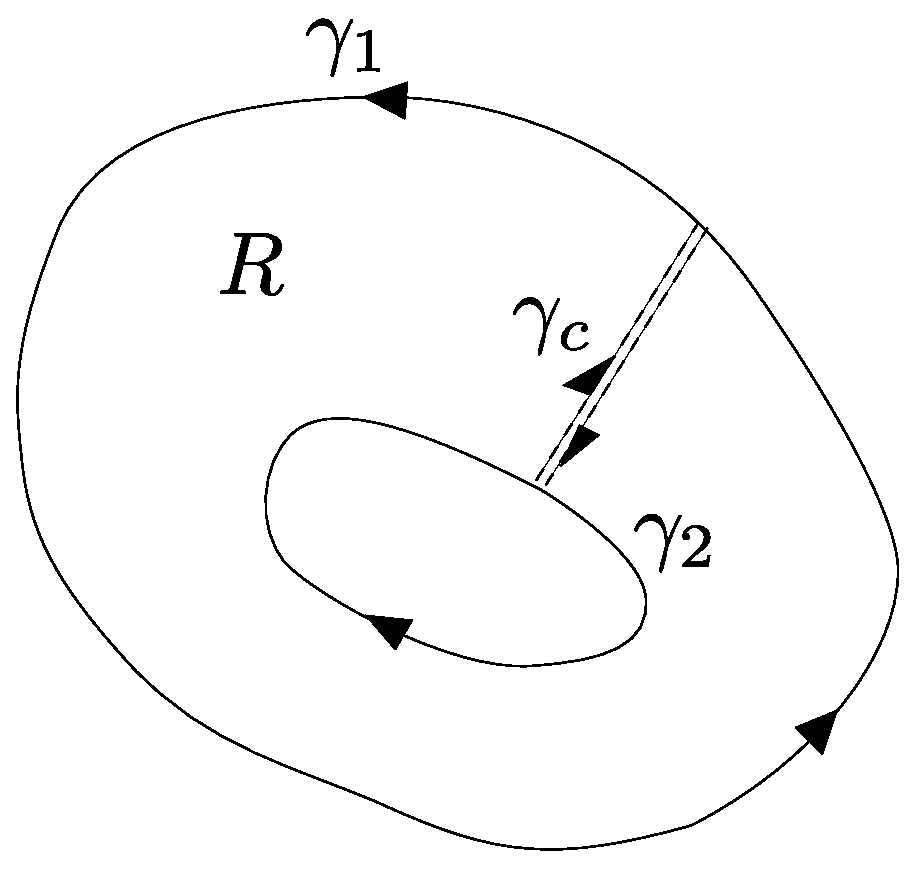
\includegraphics[width=0.30\textwidth]{./fig/nonSemplConn.eps}}
 \caption{Dominio semplice, semplicemente connesso e non semplicemente connesso.}\label{fig:green}
\end{figure}



\begin{example}
 \'E possibile calcolare l'area di una superficie $R$ tramite un integrale di linea,
 scegliendo le funzioni $P(x,y)=-\frac{1}{2}y$ e $Q(x,y)=\frac{1}{2}x$. Infatti, 
\begin{equation}
 A_R = \iint_R dx dy = \dfrac{1}{2} \oint_{\gamma_R} \left[x dy-y dx \right] .
\end{equation}
\end{example}

% +++++++++++++++++++++++++++++++++++++
\subsection{Due utili lemmi}

\begin{tabular}{cc}
\begin{minipage}{0.6\textwidth}
Il prossimo lemma è alla base dei più rinomati teoremi della divergenza e del gradiente:
 la dimostrazione di questi due teoremi si basa su un facile uso ripetuto di questo lemma.
 Data la facilità di questo lemma e la sua frequente applicazione nella scrittura di bilanci e
 in generale di integrazione per parti, è molto conveniente ricordarsi questo semplice risultato.
\begin{lemma}\label{lemma:stokes:1} Sotto le ipotesi del teorema di Green nel piano.
%\begin{empheq}[box=%
%\fbox]{align*}
\begin{equation}
  \int_V \frac{\partial A}{\partial x_i} = \oint_S A n_i
\end{equation}
%\end{empheq}
\end{lemma}
\end{minipage}
&
\begin{minipage}{0.4\textwidth}
\begin{center}
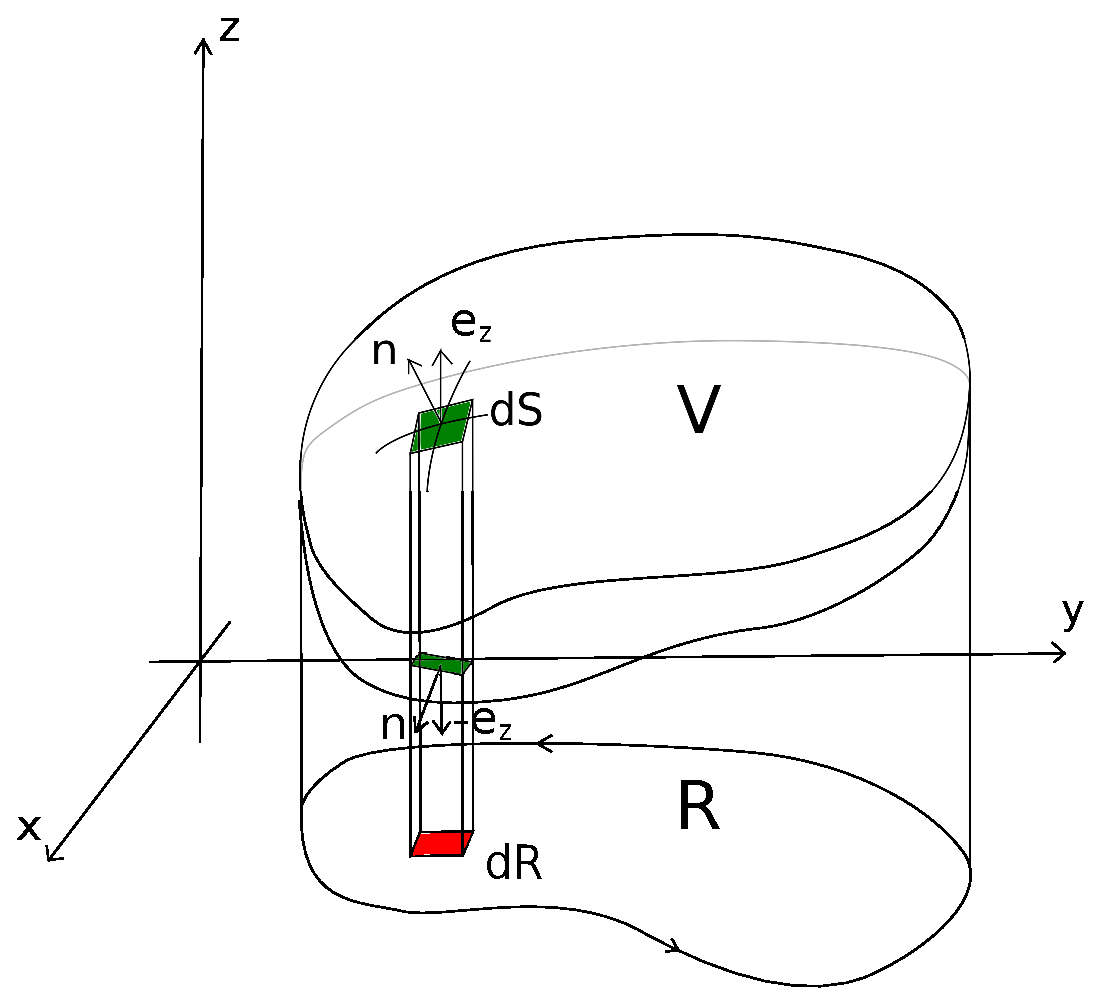
\includegraphics[width=0.95\textwidth]{./fig/Div}
\end{center}
\end{minipage}
\end{tabular}
%
\begin{proof} Si segue un ragionamento molto simile a quello utilizzato per la dimostrazione del lemma di Green nel piano.
  Per ${\partial A}/{\partial z}$:
\begin{equation}
\begin{aligned}
\int_V \frac{\partial A}{\partial z} = &
\int_R \int_{z = f_1(x,y)}^{z = f_2(x,y)} \frac{\partial A}{\partial z} dz dx dy = \\
= & \int_R [A(x,y,f_2(x,y)) - A(x,y,f_1(x,y))] dx dy %=  & (dx dy = dR = \bm{\hat{z}} \cdot \bm{\hat{n}} dS) \\
\end{aligned}
\end{equation}
%
Il passaggio più complicato è nel passare dall'integrale in $(x,y) \in R$ all'integrale sulla superficie $S$, bordo del
 volume $V$: l'elemento infinitesimo $dR$ di 
 area nel piano-xy è uguale a $dR = dx dy$; il disegno e la dimostrazione fanno riferimento a un volume \textit{semplice}
 (come nel caso di lemma di Green nel piano, è possibile generalizzare i risultati ottenuti per domini di forma generica):
 è possibile suddividere la superfice $S$ nelle due ``semisuperfici'' $S^+: z = f_2(x,y)$ e $S^- z = f_1(x,y)$ tali che
 $S^+ \cup S^- = S$ e che la normale, uscente dal volume,
 abbia componente in z positiva e negativa rispettivamente ($S^+ : \bm{\hat{n}}\cdot\bm{\hat{z}}>0$, $S^- : \bm{\hat{n}}
 \cdot\bm{\hat{z}}<0$).
La superficie elementare $dR$ è inoltre la proiezione dell'elemento di superficie $dS$ sul piano-xy: in generale $dS$ non sarà
 parallela al piano-xy e quindi sarà maggiore di $dR$. Non è difficile dimostrare che
\begin{equation}
 dx dy = dR = 
 \begin{cases}
   dS \bm{\hat{z}} \cdot \bm{\hat{n}}  & \text{su $S^+$} \\
  - dS \bm{\hat{z}} \cdot \bm{\hat{n}}  & \text{su $S^-$} \\ 
 \end{cases}
\end{equation}
Si può quindi ora continuare nella dimostrazione
\begin{equation}
\begin{aligned}
 & \int_R [A(x,y,f_2(x,y)) - A(x,y,f_1(x,y))] dx dy =   \\
 & \quad = \int_{S^+} A \bm{\hat{n}} \cdot\bm{\hat{z}} dS + \int_{S^-} A \bm{\hat{n}} \cdot\bm{\hat{z}} dS = \\
 & \quad =  \oint_S A \bm{\hat{z}} \cdot \bm{\hat{n}} dS = \\
 & \quad =  \oint_S A n_z dS
\end{aligned}
\end{equation}
\end{proof}
%\subsection*{Lemma 2}
%
\noindent 
\begin{tabular}{cc}
\begin{minipage}{0.6\textwidth}
 Come il lemma precedente è alla base della dimostrazione dei teoremi di gradiente e divergenza,
 il lemma successivo è alla base della dimostrazione del teorema del rotore.
 %
\begin{lemma} \label{lemma:stokes:2} Sotto le ipotesi del teorema di Green nel piano.
%\begin{empheq}[box=%
%\fbox]{align*}
\begin{equation}
  \int_S [\bm{\nabla} \times (A \bm{\hat{e}_i})] \cdot \bm{\hat{n}} = \oint_{\gamma} A dx_i
\end{equation}
%\end{empheq}
\end{lemma}
\end{minipage}
&
\begin{minipage}{0.4\textwidth}
\begin{center}
  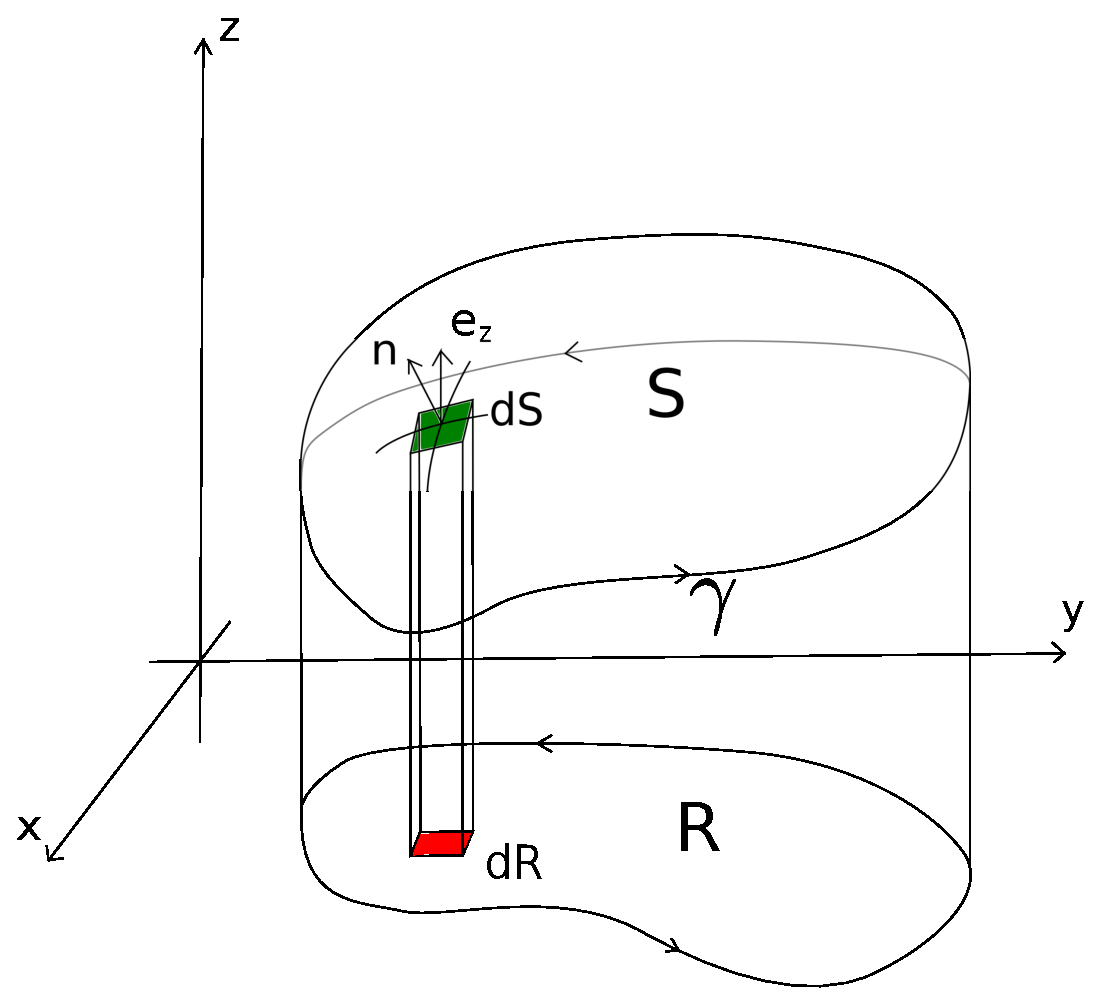
\includegraphics[width=0.95\textwidth]{./fig/Rot}
\end{center}
\end{minipage}
\end{tabular}
%
\begin{proof}
 Per $A\bm{\hat{e}_x}$, ${\nabla} \times (A \bm{\hat{e}_x}) = 
{\partial A}/{\partial z} \bm{\hat{e}_y} - {\partial A}/{\partial y} \mathbf{\hat{e}_z}$.
Si scrive la superficie S in forma parametrica come: $\bm{r} = x\bm{\hat{e}_x} +
y\bm{\hat{e}_y} + z(x,y)\bm{\hat{e}_z}$. Il vettore ${\partial \bm{r}}/{\partial y} \bm{\hat{e}_y} + 
{\partial z}/{\partial y} \bm{\hat{e}_z} $ è parallelo alla 
superficie S e quindi perpendicolare alla normale $\bm{\hat{n}}$: 
\begin{equation}
\begin{aligned}
0 = \bm{\hat{n}} \cdot \displaystyle \left(\bm{\hat{e}_y} + 
\frac{\partial z}{\partial y} \bm{\hat{e}_z} \right) \\
\end{aligned}
\end{equation}
%
Scrivendo  $[\bm{\nabla} \times (A \bm{\hat{e}_x})] \cdot \bm{\hat{n}}$:
\begin{equation}
 [\bm{\nabla} \times (A \bm{\hat{e}_x})] \cdot \bm{\hat{n}} = 
  \frac{\partial A}{\partial z} \bm{\hat{e}_y} \cdot \bm{\hat{n}}
   - \frac{\partial A}{\partial y} \bm{\hat{e}_z}\cdot \bm{\hat{n}} =
  - \displaystyle\left[ \frac{\partial A}{\partial z} \frac{\partial z}{\partial y} +
  \frac{\partial A}{\partial y}  \right] \bm{\hat{e}_z}\cdot \bm{\hat{n}}
\end{equation}
%
Se si riconosce ${\partial A(x,y,z(x,y))}/{\partial y} = {\partial A}/{\partial z} {\partial z}/{\partial y} +
  {\partial A}/{\partial y}$, si può scrivere:
\begin{equation}
 \int_S [\bm{\nabla} \times (A \bm{\hat{e}_x})] \cdot \bm{\hat{n}} =
 - \int_S \frac{\partial A}{\partial y} \underbrace{\bm{\hat{e}_z}\cdot \bm{\hat{n}} dS}_{dR = dx dy} = 
 - \int_R \frac{\partial A}{\partial y} dx dy = \int_\gamma A dx
\end{equation}
%
\end{proof}


% +++++++++++++++++++++++++++++++++++++
\subsection{Teorema della divergenza, del rotore e del gradiente}
Vengono ora enunciati i teoremi della divergenza, del rotore e del gradiente. Senza entrare nei dettagli delle ipotesi dei teoremi, affinchè i loro enunciati siano validi, gli oggetti matematici coinvolti devono almeno esistere. L'ipotesi di ``sufficiente regolarità'' dei campi vettoriali viene tradotta volgarmente nel comportamento regolare della funzione all'interno del dominio, che esclude l'esistenza di poli (punti del dominio in cui funzione tende all'infinito) e comprende l'esistenza (e la continuità) delle derivate spaziali del campo.
%
%Non si presterà qui molta
% attenzione alle ipotesi di tali teoremi, ma si ricordi che alcuni accorgimenti devono essere usati nel caso di domini
% non semplicemente connessi e che \textbf{gli oggetti contenuti nei teoremi devono almeno esistere} (vago riferimento alle condizioni
% di differenziabilità dei campi) affinchè i teoremi siano validi.

Per far intuire l'utilità dei due lemmi presentati in precedenza, si riportano anche le dimostrazioni dei teoremi: una volta noti i due utili(ssimi) lemmi, queste dimostrazioni sono così immediate da occupare soltanto una riga.

%\subsection*{Teorema della divergenza}
\begin{theorem}\label{thm:grad}[Teorema della divergenza] Si consideri un insieme $V \subset R^n$ compatto delimitato da una superficie liscia $S = \partial V$. Se $\mathbf{v}$ è un campo vettoriale differenziabile con continuità (di classe $C^1$) definito in un intorno di V, allora
\begin{equation}
  \int_V \bm{\nabla} \cdot \bm{v} = \oint_S \bm{v} \cdot \hat{\bm{n}} ,
\end{equation}
 essendo $\bh{n}$ la normale alla superficie $S$ uscente dal volume $V$.
\end{theorem}

\begin{proof}
Il teorema viene dimostrato scrivendo la divergenza in un sistema di coordinate cartesiane, $\bm{\nabla} \cdot \bm{v} = \sum_i \frac{\partial v_i}{\partial x_i}$, e applicando il lemma \ref{lemma:stokes:1} a ogni derivata parziale nella sommatoria,
\begin{equation}
\int_V \bm{\nabla} \cdot \bm{v} = 
  \int_V \sum_i \frac{\partial v_i}{\partial x_i} = \oint_S \sum_i v_i n_i = \oint_S \bm{v} \cdot \bm{\hat{n}} .
\end{equation}
\end{proof}

%\subsection*{Teorema del rotore}
\begin{theorem}[Teorema del rotore] In maniera abbastanza generale, sotto le ipotesi dei teoremi precedenti, vale
\begin{equation}
  \int_S [\bm{\nabla} \times \bm{v}] \cdot \bm{\hat{n}} = \oint_{\gamma} \bm{v} \cdot \bh{t} ,
\end{equation}
  avendo omesso l'elemento di lunghezza $d\ell$ nell'integrale di linea e avendo indicato con $\bh{t}$ il versore tangente alla curva $\gamma$.
\end{theorem}

\begin{proof}
Il teorema viene dimostrato utilizzando un sistema di coordinate cartesiane e applicando il lemma \ref{lemma:stokes:2} a ogni componente del vettore $\bm{v} = v_x \bm{\hat{e}_x} + v_y \bm{\hat{e}_y} + v_z \bm{\hat{e}_z} = \sum_i v_i \bm{\hat{e}_i}$,
\begin{equation}
\int_S [\bm{\nabla} \times \bm{v}] \cdot \bm{\hat{n}} = 
\int_S \Big[\bm{\nabla} \times \Big(\sum_i v_i \bm{\hat{e}_i}\Big)\Big] \cdot \bm{\hat{n}} =
\int_{\gamma} \sum_i v_i dx_i = \int_{\gamma} \bm{v} \cdot d\bm{l} =
\int_{\gamma} \sum_i v_i dx_i = \int_{\gamma} \bh{t} ,
\end{equation}
 avendo utilizzato le coordinate cartesiane e la definizione di versore tangente per esprimere l'elemento di lunghezza, $d\bm{l} = dx \bh{x} + dy \bm{y} + dz \bh{z} = \bh{t} ds$.
\end{proof}

%\subsection*{Teorema del gradiente}
\begin{theorem}[Teorema del gradiente] In maniera abbastanza generale, sotto le ipotesi dei teoremi precedenti, per un campo scalare $f$ sufficientemente regolare vale
\begin{equation}
  \int_V \bm{\nabla} f = \oint_S f \hat{\bm{n}} .
\end{equation}
\end{theorem}

\begin{proof}
Il teorema viene dimostrato scrivendo il gradiente del campo scalare $f$ in coordinate cartesiane, $\bm{\nabla} f = \sum_i \frac{\partial f}{\partial x_i} \bm{\hat{e}_i}$, e applicando il lemma \ref{lemma:stokes:1} a ogni derivata parziale nella sommatoria,
\begin{equation}
\int_V \bm{\nabla} f = 
  \int_V \sum_i \frac{\partial f}{\partial x_i} \bm{\hat{e}_i} =
   \oint_S \sum_i f n_i \bm{\hat{e}_i} = \oint_S f \bm{\hat{n}} .
\end{equation}
\end{proof}
%
Prima di continuare i richiami di analisi, viene fatta un'osservazione sulla notazione usata.
\begin{remark}
 Per indicare gli integrali di linea, superficie e volume verrà omesso l'elemendo infinitesimo di linea, superficie e volume, indicando il dominio di integrazione di fianco al segno di integrale. In maniera esplicita l'integrale sulla linea $\ell$ , sulla superficie $S$ e sul volume $V$ di una quantità scalare $f$ verranno indicati semplicemente con
 \begin{equation}
  \int_{\ell} f , \quad \int_S f , \quad \int_V f .
 \end{equation}
 Il valore di un integrale è indipendente dalle coordinate utilizzate per svolgerlo. Per calcolare il valore dell'integrale è necessario introdurre un sistema di coordinate per parametrizzare in una maniera conveniente la funzione, il dominio e gli elementi infinitesimi di lunghezza, superficie o volume. Spesso questa scelta può essere dettata dalla geometria del dominio.
Per completezza vengono riportate epslicitamente le espressioni degli elementi infinitesimi di:
\begin{itemize}
\item lunghezza (con versore tangente) della curva $\ell$, descritta dalla parametrizzazione $\ell: \bm{r} = \bm{r}(l) =  \bm{r}(l(s)) = \bm{\tilde{r}}(s)$,
 \begin{equation}
  d \bm{r} = \dfrac{d \bm{r}}{d l} d l = \underbrace{\dfrac{d \bm{r}}{d s}}_{\bh{t}} d s = \bh{t} \ ds ,
 \end{equation}
 avendo riconosciuto il versore $\bh{t}$ tangente alla curva, introdotto l'ascissa curvilinea $s$, e indicato con $\bm{r}(l)$ la parametrizzazione in funzione di $l$ e con $\bm{\tilde{r}}(s)$ la parametrizzazione in funzione di $s$.
\item di superficie (con versore normale) della superficie bidimensionale $S$, descritta dalla parametrizzazione $S: \bm{r} = \bm{r}(u,v)$,
 \begin{equation}
  \bh{n} \ dS = \p{\bm{r}}{u} \times \p{\bm{r}}{v} du dv
 \end{equation}
\item di volume del volume tridimensionale $V$, descritto dalla parametrizzazione dello spazio $V: \bm{r} = \bm{r}(u,v,w)$,
\begin{equation}
 dV = \p{\bm{r}}{u} \cdot  \p{\bm{r}}{v} \times \p{\bm{r}}{w} du dv dw .
\end{equation}
\end{itemize} 
Si fanno quindi alcuni esempi. 
\begin{example}\label{exa:pol:line}
Si vuole calcolare l'elemento infinitesimo di curva di una circonferenza $C$ di raggio $R$. Si utilizza un sistema di riferimento cartesiano con origine nel centro della circonferenza e l'angolo $\theta$ che il vettore posizione $\bm{r}$ forma con l'asse $x$ per parametrizzare la curva
\begin{equation}
  C : \ \bm{r}(\theta) = x(\theta) \bh{x} + y(\theta) \bh{y} = R \cos \theta \bh{x} + R \sin \theta \bh{y} .
\end{equation}
L'elemento di curva $d \bm{r}$ risulta
\begin{equation}
 d\bm{r} = \dfrac{d\bm{r}}{d \theta} = \left( -\sin \theta \bh{x} + \cos \theta \bh{y} \right) R d \theta = \bh{\theta} R d\theta = \bh{\theta} ds ,
\end{equation}
avendo introdotto l'ascissa curvilinea $s = R \theta$ e il versore $\bh{\theta}$ tangente alla circonferenza.
\end{example}
% ----
\begin{example}\label{exa:cyl:surf}
Si vuole calcolare la superficie elementare (con versore normale) di una superficie sferica $S$ parametrizzata con gli angoli $\varphi$ e $\theta$,
\begin{equation}
\begin{aligned}
 \bm{r}(\varphi,\theta) & = 
 x(\varphi,\theta) \bh{x} + y(\varphi,\theta) \bh{y} + z(\varphi,\theta) \bh{z} = \\
& = R \sin \varphi \cos \theta \bh{x} +
    R \sin \varphi \sin \theta \bh{y} +
    R \cos \varphi \bh{z} .
\end{aligned}
\end{equation}
Da un calcolo diretto, senza riportare tutti i passaggi, si ottiene
\begin{equation}
\begin{aligned}
 \bh{n} dS & = \p{\bm{r}}{\varphi} \times \p{\bm{r}}{\theta} d\varphi d\theta = \\
 & = \left( \sin \varphi \cos \theta \bh{x} + \sin \varphi \sin \theta \bh{y} + \cos \varphi \bh{z} \right) R^2 \sin \varphi d \varphi d \theta = \\
 & = \bh{R} R^2 \sin \varphi d \varphi d \theta .
\end{aligned}
\end{equation}
\end{example}
% ----
\begin{example}\label{exa:cyl:vol}
Si vuole calcolare il volume elementare di una volume $V$ parametrizzato in coordinate sferiche, cioè con il raggio $R$ e gli angoli $\varphi$ e $\theta$,
\begin{equation}
\begin{aligned}
 \bm{r}(\varphi,\theta) & = 
 x(R,\varphi,\theta) \bh{x} + y(R,\varphi,\theta) \bh{y} + z(R,\varphi,\theta) \bh{z} = \\
& = R \sin \varphi \cos \theta \bh{x} +
    R \sin \varphi \sin \theta \bh{y} +
    R \cos \varphi \bh{z} .
\end{aligned}
\end{equation}
Da un calcolo diretto, senza riportare tutti i passaggi, si ottiene
\begin{equation}
\begin{aligned}
 dV & = \p{\bm{r}}{R} \cdot \p{\bm{r}}{\varphi} \times \p{\bm{r}}{\theta} dR d\varphi d\theta = \\
  & = \bh{R} \cdot \bh{R} R^2 \sin \varphi dR d \varphi d \theta = \\
  & = R^2 \sin \varphi dR d \varphi d \theta .
\end{aligned}
\end{equation}
\end{example}

\begin{figure}[h]
\centering
%\captionsetup[subfigure]{labelformat=empty}
\subfloat[][\emph ]
   {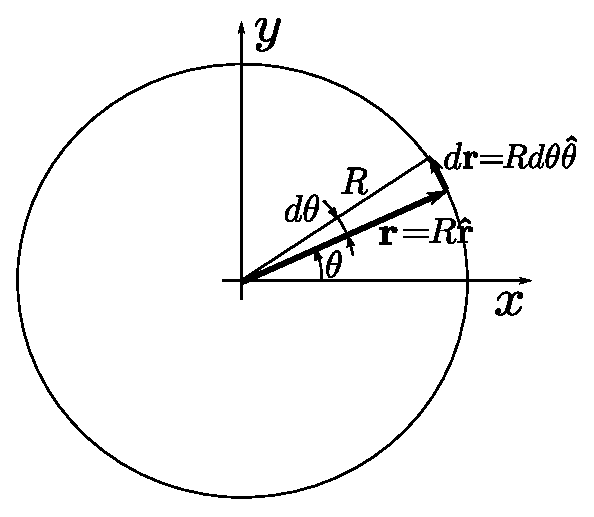
\includegraphics[width=0.50\textwidth]{./fig/circle.eps}\label{fig:elementary:circle}} \quad
\subfloat[][\emph ]
   {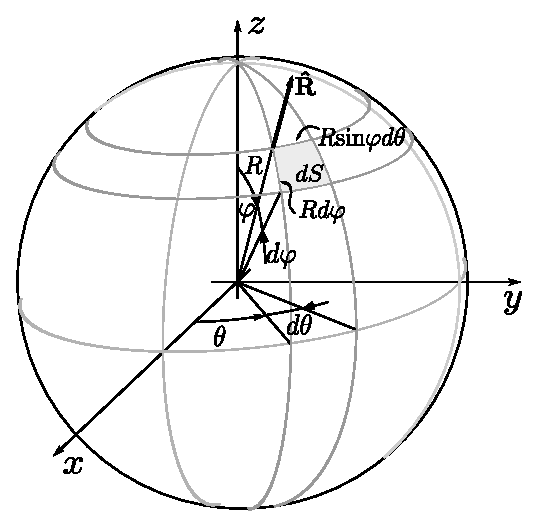
\includegraphics[width=0.45\textwidth]{./fig/sphere.eps}\label{fig:elementary:sphere}}
\caption{Sistemi di coordinate usati negli esempi \ref{exa:pol:line}-\ref{exa:cyl:vol}. \protect\subref{fig:elementary:circle} Coordinate polari. \protect\subref{fig:elementary:sphere} Coordinate sferiche.}\label{fig:elementary} 
\end{figure}

\end{remark} 

% --------------------------------------------------------------------------------------------------

\section{Campi vettoriali conservativi}

In alcuni casi l'integrale $I = \int_\gamma \bm{F} \cdot \bh{t}$ è indipendente dal percorso di integrazione $\gamma$. L'indipendenza del valore dell'integrale $I$ da $\gamma$ è strettamente collegata all'idea di differenziale esatto: quando $I$ è indipendente da $\gamma$, ma dipende solo dai suoi estremi $a$, $b$, si può scrivere $I = \int_\gamma \bm{F} \cdot \bh{t} = \int_a^b d\phi = \phi(b) - \phi(a)$. Se l'integrale di linea $I$ su ogni curva nel dominio $V$ dipende solo dagli estremi di integrazione, il campo vettoriale $\bm{F}$ viene definito \textbf{conservativo}.

\noindent	
L'indipendenza del valore dell'integrale dal percorso di integrazione ha alcune conseguenze:
\begin{itemize}
\item l'integrale su ogni percorso chiuso è nullo: $\oint_{l} \bm{F} \cdot d\bm{r} = 0$;
\item il campo $\bm{F}$ può essere scritto come gradiente di una funzione scalare $\phi$, che assume
      il significato di potenziale: $\bm{F} = \bm{\nabla}\phi$;
\item il rotore del campo vettoriale è nullo: $\bm{\nabla} \times \bm{F} = 0$ (infatti $\bm{\nabla} \times \bm{\nabla} \phi= 0$,
 per ogni funzione scalare $\phi$).
\end{itemize}
%
Le condizioni elencate sono quindi \textbf{condizioni necessarie} per l'indipendenza dell'integrale dal percorso di integrazione.
Se prese a se stanti, esse non sono anche condizioni sufficienti. Affinchè la seconda e la terza condizione siano
anche sufficienti, è necessario che il dominio sia semplicemente connesso.
